\documentclass[10pt, letterpaper]{article}
\usepackage{graphicx}
\usepackage[bottom=1.0in]{geometry}
\topmargin=-0.9in
\oddsidemargin -.3in
\evensidemargin -0.3in
\textwidth=7.0in
%\itemsep= -0.5in
%\parsep= -0.04in

\usepackage[cmex10]{amsmath}
\usepackage{multirow}



\author{Madhusudan Govindraju 39267182 }
\date{}
\begin{document}
\title{EEL5840  Elements of Machine Intelligence - HW 2}
\maketitle

The steps done to solve the assignment has been outlined in detail along with the assumptions and the data used.


First during the training phase, we calculate the optimal weights W from the training data, using the formula $$ W = {R}^{-1} * P $$  where $$ R = XX^{T} $$ $$P = X^{T}Y$$ For this step we use the following set of  hyperparameters($\lambda$) and filter orders. 


\begin{table}[h!]
\begin{center}
\caption{Filter Orders and $\lambda$ used}
\label{table:hyper_parameters}
\begin{tabular}{ |c|c|c|c|c|c| }
\hline
\hline
Filter Order	& 4		& 8 		& 15 		& 25 		&30 \\
\hline
$\lambda$		&0.001 	& 0.020 	&0.04 	& 0.08 	&0.1\\
\hline
\end{tabular}
\end{center}
\end{table}

The other assumption is that the input is a time series with 1feature per sample and there are $N$ samples. where $N=3000$ in training $N=1000$ in validation \& test. 

The following experiments are done with the above mentioned assumptions
%\begin{table}[h!]
%\centering
%\caption{The W and MSE obtained for different the different filter orders and $\lambda$ values}
%\label{table:W&MSE}
%\begin{tabular} {|c|c|c|c|c|}
%\hline
%S.No		&Filter Order 	& Lambda 		& W 				& MSE			\\
%\hline
%1		&4			&1.000000e-03		&9.960486e-01		&1.361874e-05		\\
%2		&4			&2.000000e-02		&9.960413e-01		&1.366958e-05		\\
%3		&4			&4.000000e-02		&9.960335e-01		&1.372321e-05		\\
%4		&4			&8.000000e-02		&9.960180e-01		&1.383077e-05		\\
%5		&4			&1.000000e-01		&9.960102e-01		&1.388471e-05		\\
%6		&8			&1.000000e-03		&9.881238e-01		&1.224466e-04		\\
%7		&8			&2.000000e-02		&9.881164e-01		&1.225974e-04		\\
%8		&8			&4.000000e-02		&9.881088e-01		&1.227562e-04		\\
%9		&8			&8.000000e-02		&9.880934e-01		&1.230742e-04		\\
%10		&8			&1.000000e-01		&9.880857e-01		&1.232333e-04		\\
%11		&15			&1.000000e-03		&9.677785e-01		&8.954667e-04		\\
%12		&15			&2.000000e-02		&9.677713e-01		&8.958647e-04		\\
%13		&15			&4.000000e-02		&9.677638e-01		&8.962838e-04		\\
%14		&15			&8.000000e-02		&9.677487e-01		&8.971222e-04		\\
%15		&15			&1.000000e-01		&9.677412e-01		&8.975415e-04	\\
%16		&25			&1.000000e-03		&9.342439e-01		&3.699135e-03		\\
%17		&25			&2.000000e-02		&9.342370e-01		&3.699913e-03		\\
%18		&25			&4.000000e-02		&9.342298e-01		&3.700731e-03		\\
%19		&25			&8.000000e-02		&9.342152e-01		&3.702369e-03		\\
%20		&25			&1.000000e-01		&9.342079e-01		&3.703188e-03		\\
%21		&30			&1.000000e-03		&9.182905e-01		&5.686370e-03		\\
%22		&30			&2.000000e-02		&9.182837e-01		&5.687316e-03		\\
%23		&30			&4.000000e-02		&9.182766e-01		&5.688311e-03		\\
%24		&30			&8.000000e-02		&9.182623e-01		&5.690303e-03		\\
%25		&30			&1.000000e-01		&9.182551e-01		&5.691298e-03		\\
%\hline
%\end{tabular}
%\end{table}








\begin{enumerate}
\item  We use the above mentioned formula to calculate the optimal weight for the validation data set. The set of optimal weights W obtained for the following filter orders and  $\lambda$ is shown in table \ref{table:W&MSE} , along wth the Mean Squared Error obtained.

With the hyper parameter, filter order and optimal weights obtained from the step above,
%, we use the formula   $MSE = mean((Y - \overline{Y})^{2})$ 
to calculate the mean squared error. where $Y$ is the desired output and $\overline{Y}$ is the obtained output. This is implemented on the validation data set to obtain the MSE.

The table \ref{fig:MSE_Table} shows us the MSE obtained for the different values of filter order and $\lambda$.



\begin{figure}
\centering
\label{fig:PerformancePlot}
\caption{Performance Plot}
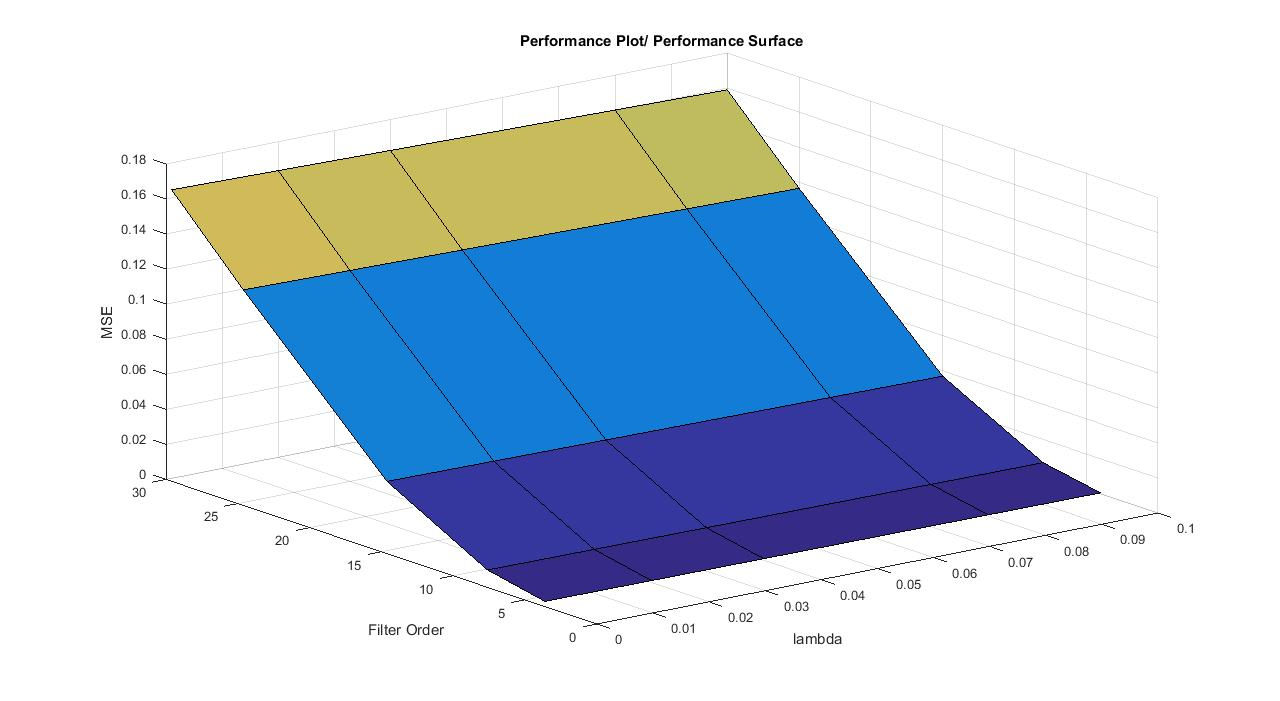
\includegraphics[scale=0.25]{PerformancePlot}
\end{figure}

\begin{figure}
\centering
\label{fig:MSE_Table}
\caption{Table :For MSE over different hyper parameters}
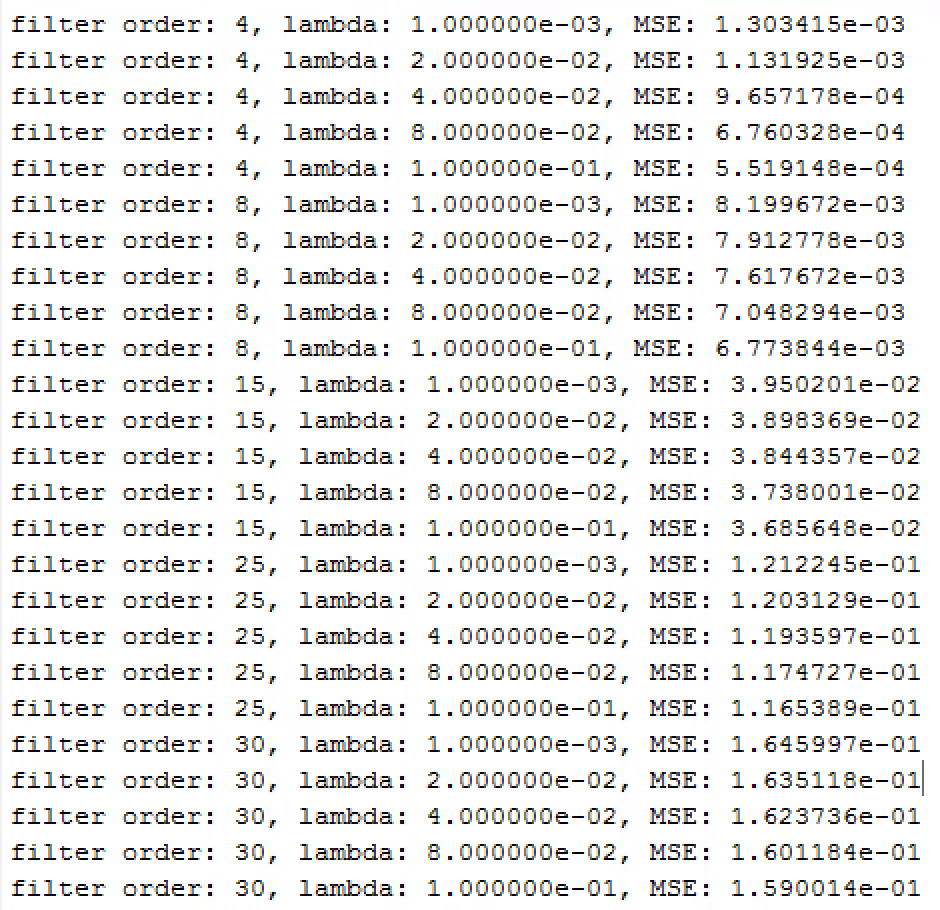
\includegraphics[scale=1]{table}
\end{figure}

We plot a 3D surface plot - the performance pot as shown in figure\ref{fig:PerformancePlot}
From these values of MSE we choose the lowest point in the surface which will correspond to the best Weight, hyper parameter and the filter order. We proceed to use those selected values on the test data set to check the error obtained though time. The point with the lowest point in the surface plot in figure  \ref{fig:PerformancePlot} will be the optimum point. That is called the local minimum(or even Global minimum in this case).

From figure 2 we choose the parameters that give the best performance to test on the test.mat data. 

The best performance is obtained with the following parameters, filter order: 4, lambda: 1.000000e-01, MSE: 5.519148e-04

\item We now use these parameters and run it on the test.mat data and calculate the MSE obtained. 
The MSE obtained for different filter orders are as follows \\
$filter order: 4 - MSE: 3.811019e+00$ \\
$filter order: 8 - MSE: 2.046562e+01$ \\
$filter order: 30 - MSE: 3.390014e+02$

The figures 3,4,5 depict the errors obtained vs input over time.
\begin{figure}
\centering
\label{fig:four}
\caption{For Filter order 4}
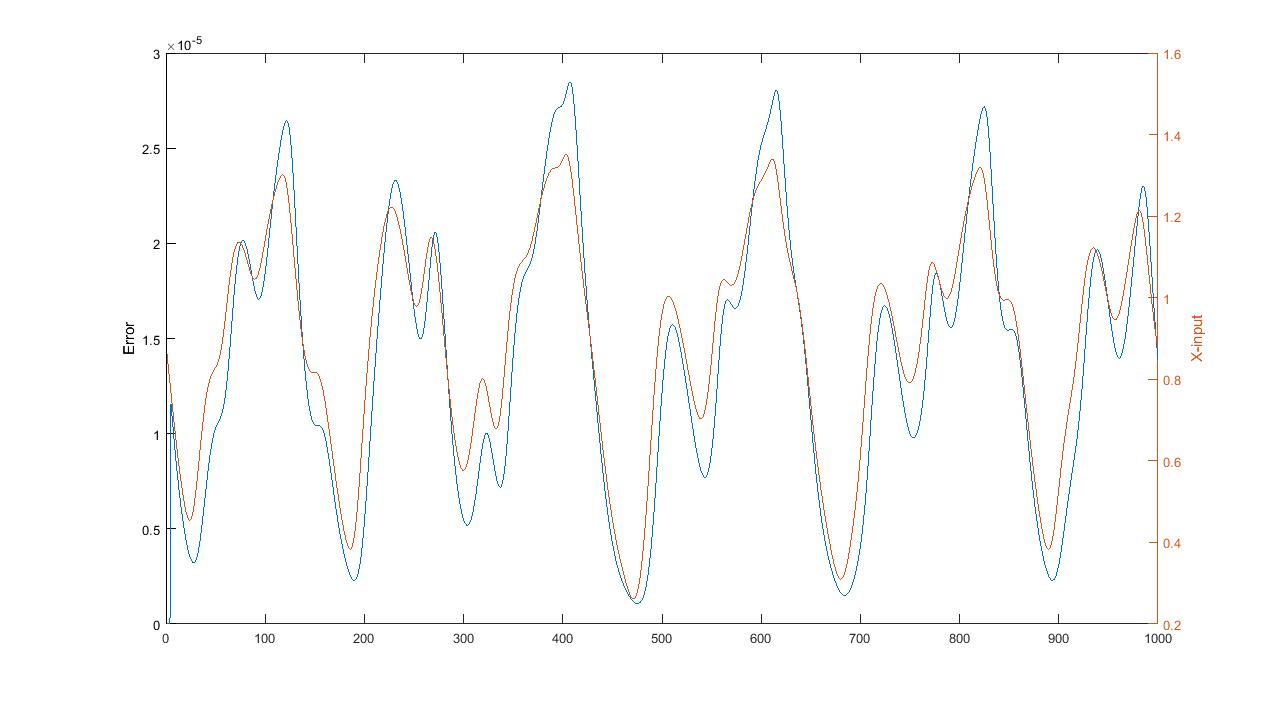
\includegraphics[scale=0.25]{MSE}
\end{figure}
\begin{figure}
\centering
\label{fig:eight}
\caption{For Filter order 8}
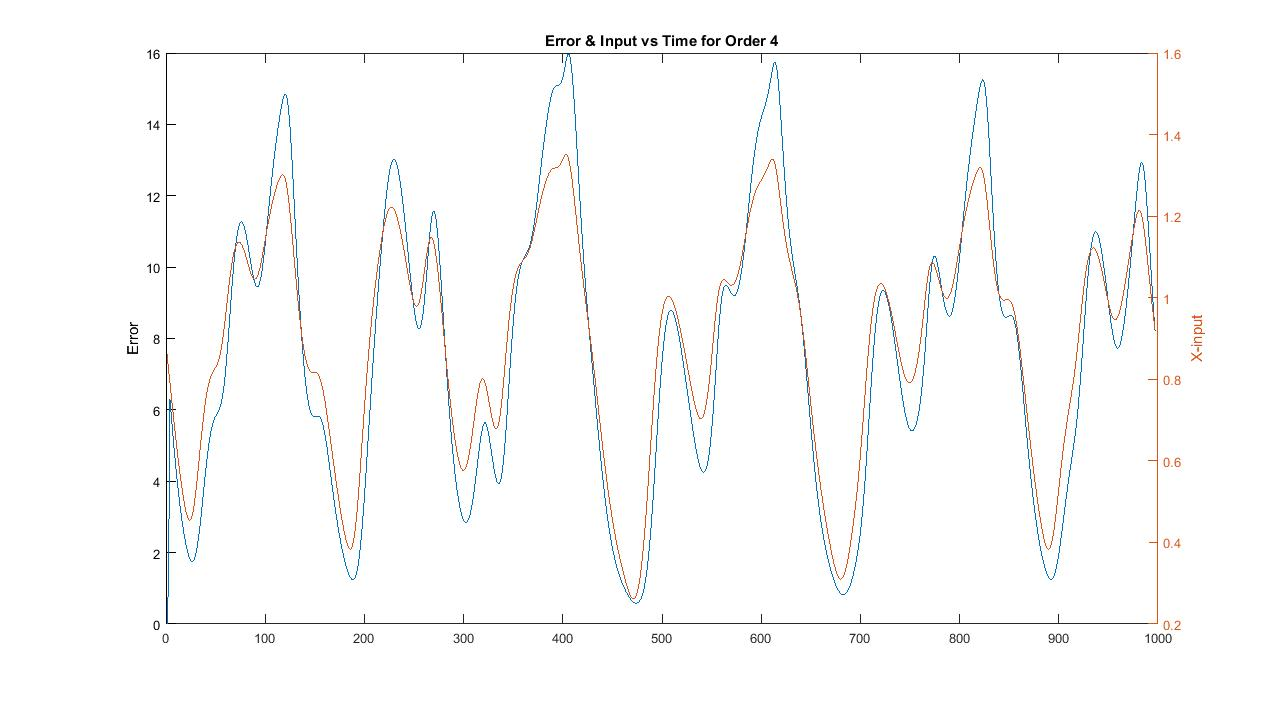
\includegraphics[scale=0.25]{MSE1}
\end{figure}
\begin{figure}
\centering
\label{fig:thirty}
\caption{For Filter order 30}
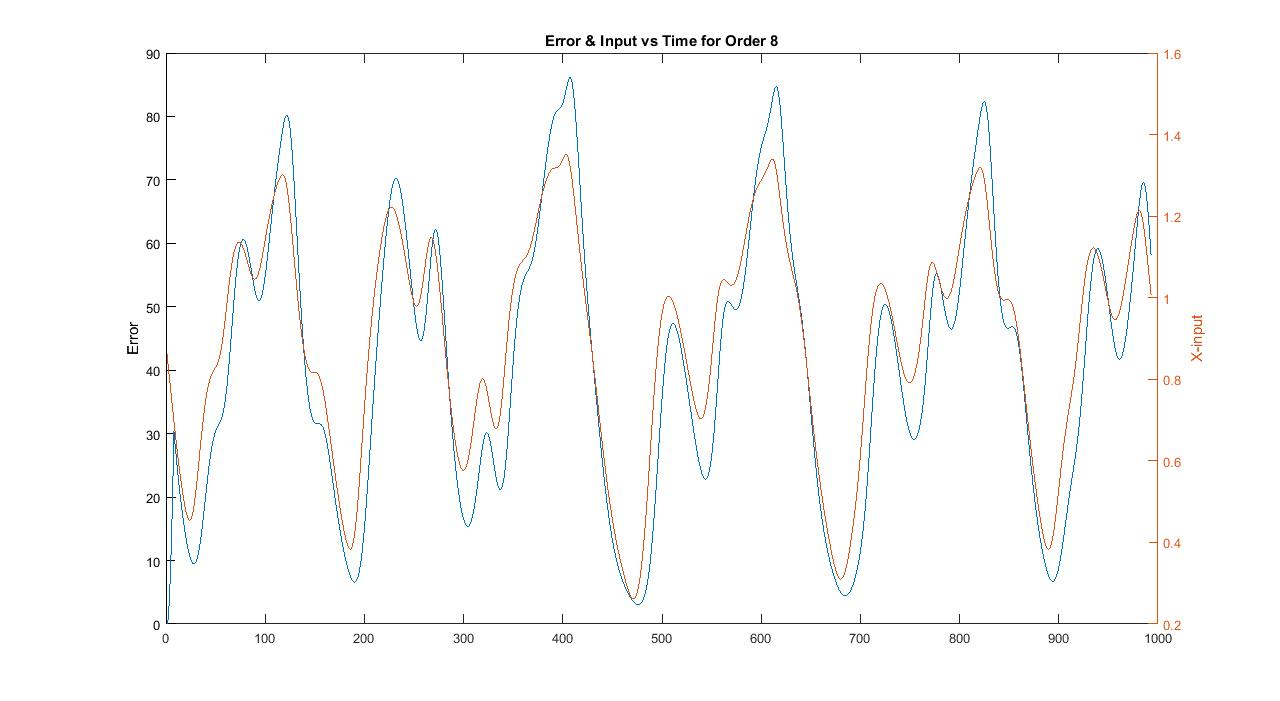
\includegraphics[scale=0.25]{MSE2}
\end{figure}

If we notice the error it changes in accordance to the amplitude of the input signal, hence it is not constant over time. The variation of the square error "is a quadratic function of the deviation of the weight parameters and depends only on the input signal statistics"(from lecture slide), this explains the variation of the error across time.
 
 
 \item Now the same is done for the Noisy data in the file testnoisy.mat. The $\lambda$ which has the least value is chosen for the order and the error is plotted over time. Because this is a noisy signal there are a lot of peaks. The figures 6,7,8 depict the errors obtained vs input over time. The figures 6,7,8 are not clear hence the figures 9\&10 are given for easy understand of the system
\begin{figure}
\centering
\label{fig:four1}
\caption{For Filter order 4 - Noisy Signal}
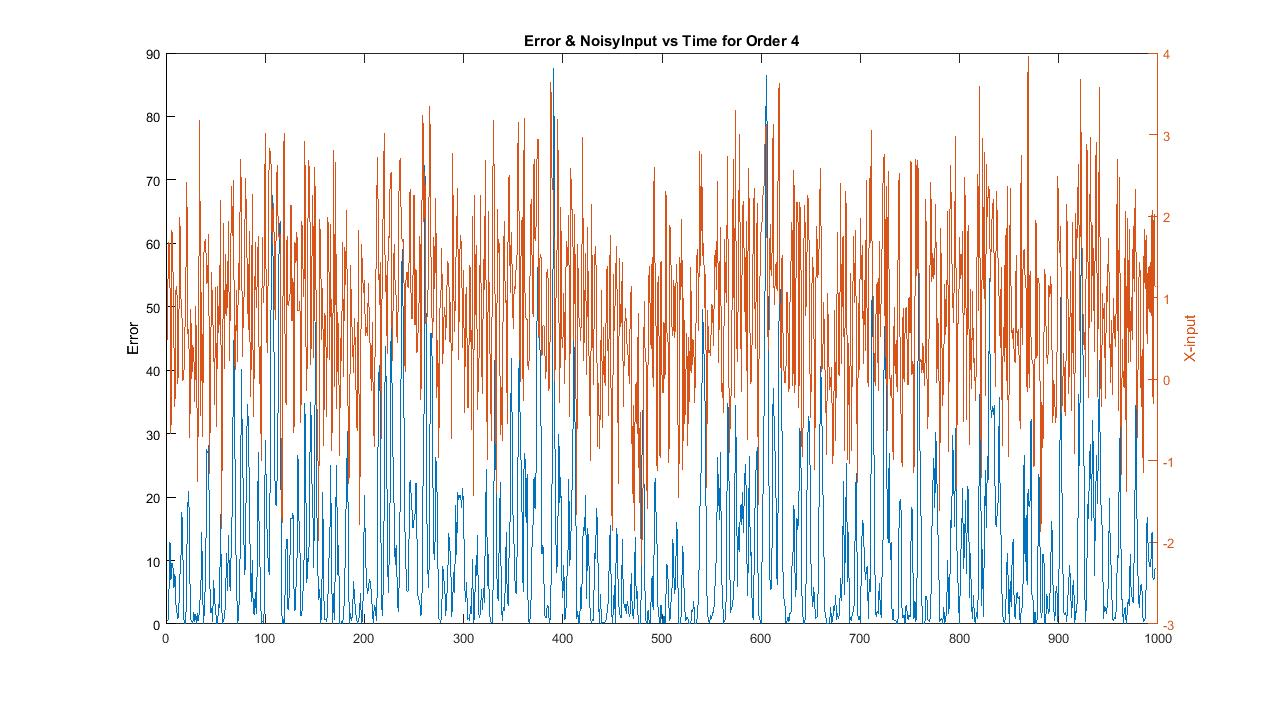
\includegraphics[scale=0.25]{MSE1_Noisy}
\end{figure}
\begin{figure}
\centering
\label{fig:eight1}
\caption{For Filter order 8 - For noisy Signal}
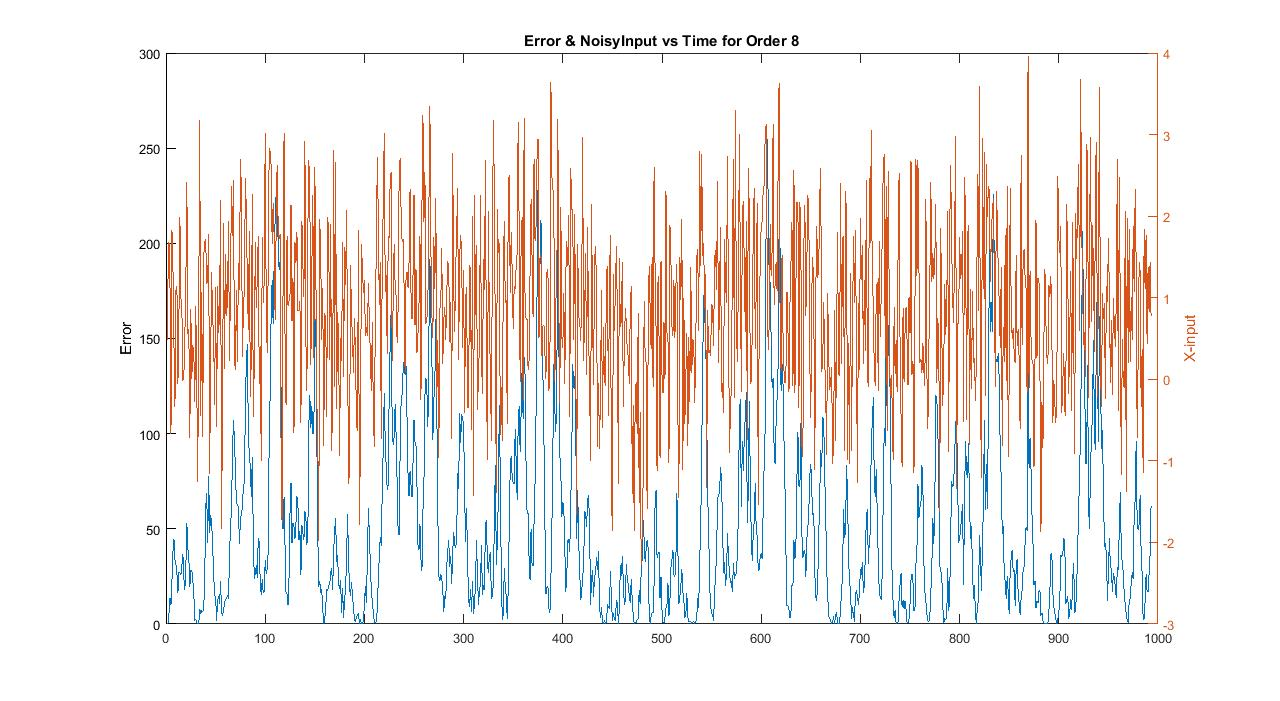
\includegraphics[scale=0.25]{MSE2_Noisy}
\end{figure}
\begin{figure}
\centering
\label{fig:thirty1}
\caption{For Filter order 30 - For noisy Signal}
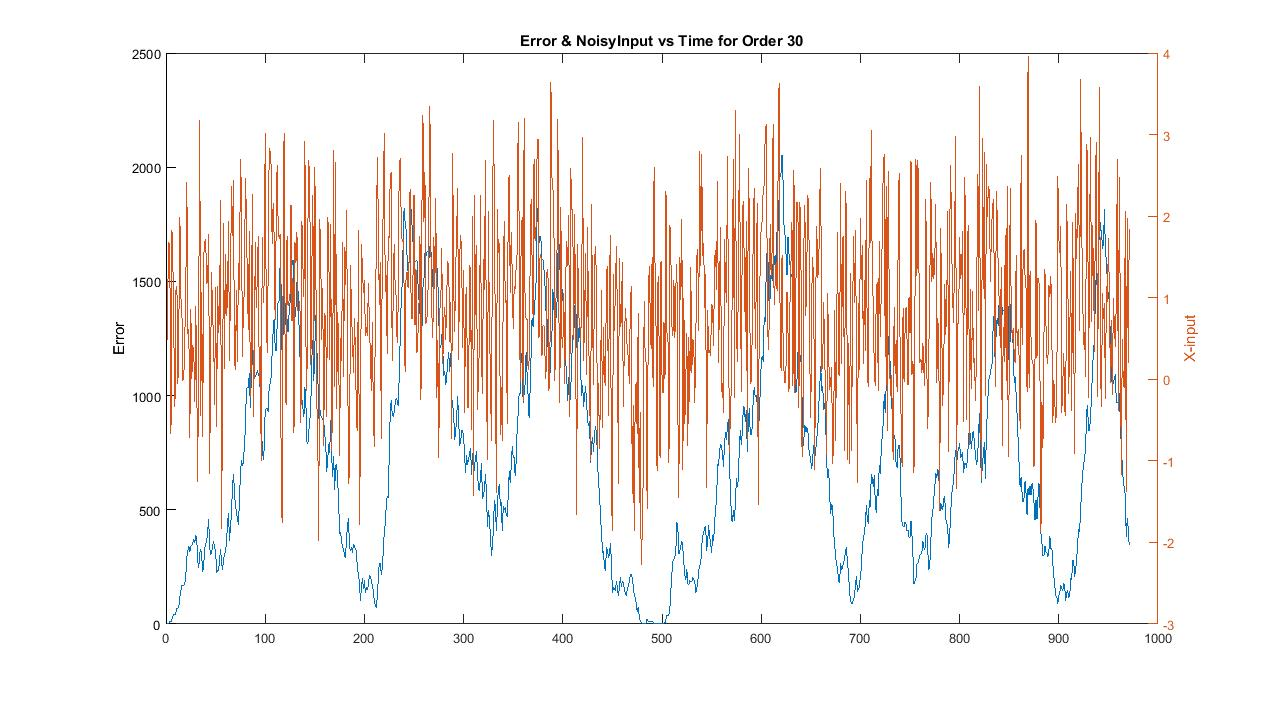
\includegraphics[scale=0.25]{MSE3_Noisy}
\end{figure}

The figure 9 compares the errors obtained for the three orders 
\begin{figure}
\centering
\label{fig:ErrorComparison}
\caption{Comparison of Errors for the Different Orders on the Noisy Signal}
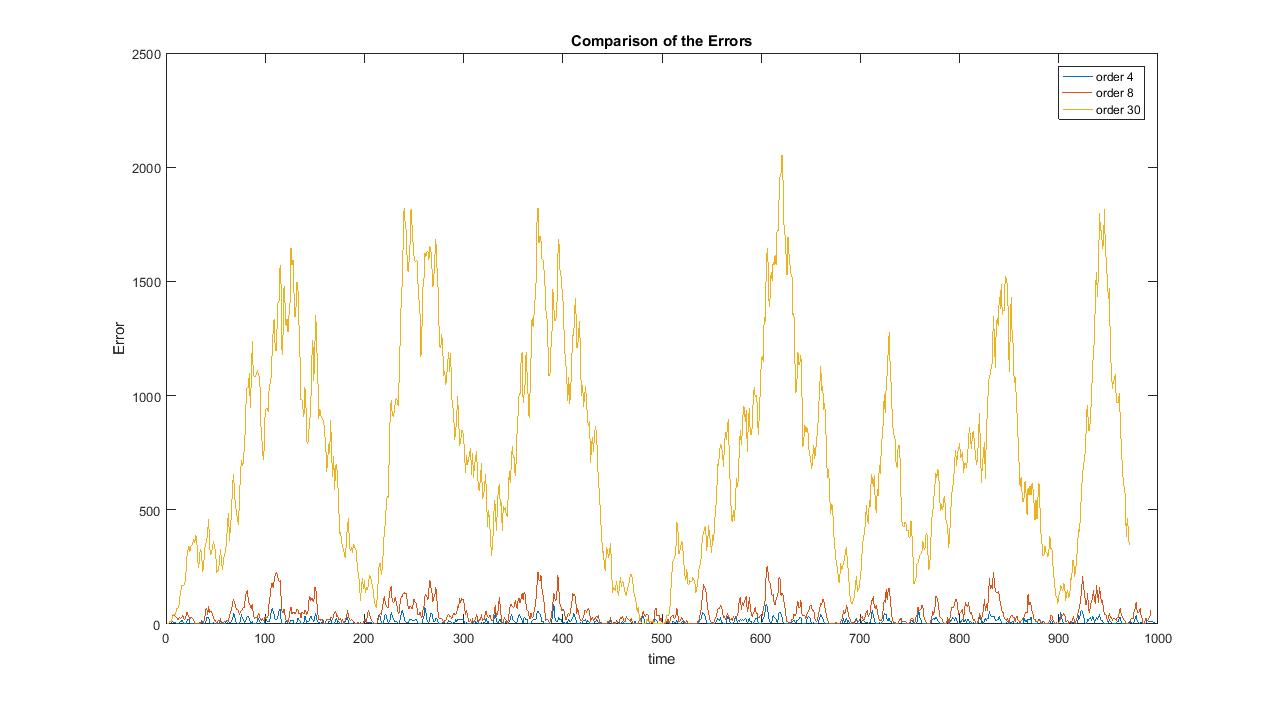
\includegraphics[scale=0.25]{ComparisonOfErrors.jpg}
\end{figure}

The figure 10 plots the Average Error obtained over time for the noisy signal over the different orders
\begin{figure}
\centering
\label{fig:AvgErrorComparison}
\caption{Avg Error over the time range for the noisy signal for different orders}
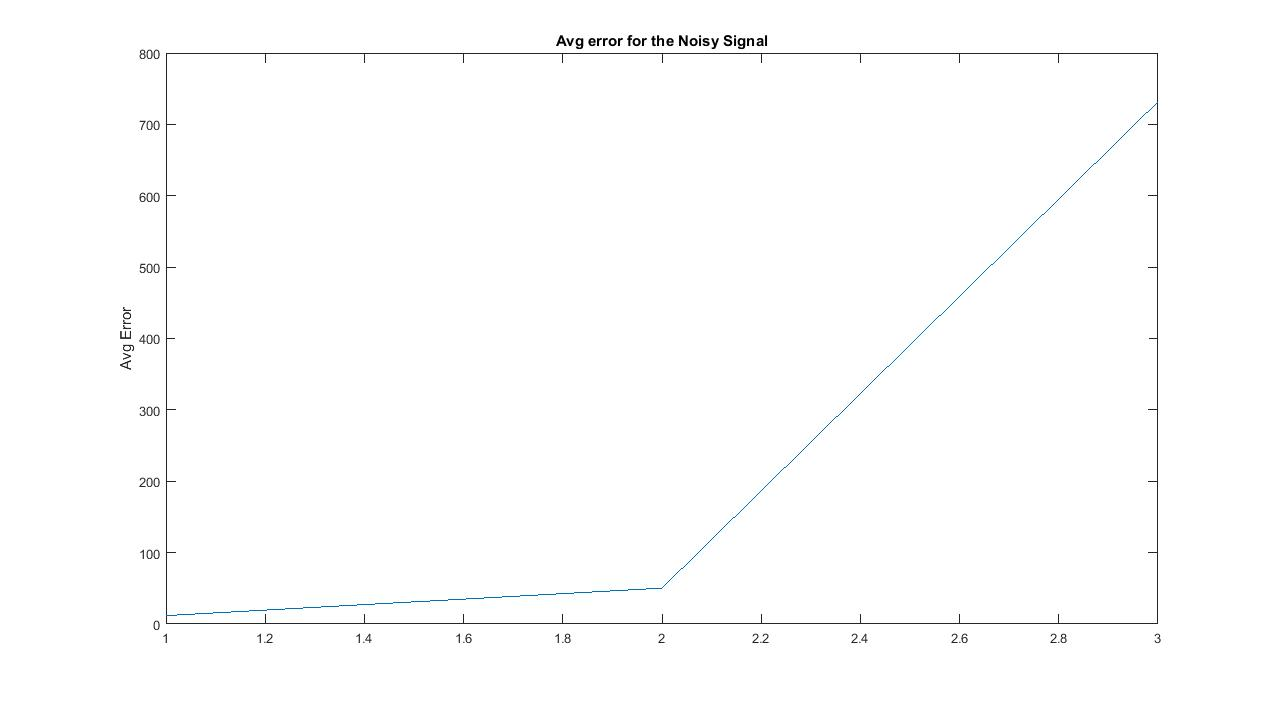
\includegraphics[scale=0.25]{AvgErrorForNoisySignal.jpg}
\end{figure}

From Figure 9 and Figure 10 we can clearly understand that the system with order 4 has the least error. Hence choosing order four will have better characteristics. Because we are dealing with a convex error surface, the least error will be at the local minimum, so the order and the $\lambda$ which gives the least error will perform best for the system. In the figure one we can see that the least error is obtained for order 4 so the even the noisy system performs better for order 4

For noisy data\\
filter order: 4, lambda: 1.000000e-01, MSE: 5.879905e+00\\
filter order: 8, lambda: 1.000000e-01, MSE: 2.513405e+01\\
filter order: 30, lambda: 1.000000e-01, MSE: 3.658688e+02\\

\end{enumerate}



\end{document}